\section{Use Cases for Source Coverage Ratio}
\label{sec:apps}

This section returns to the sample queries of Section~\ref{sec:qtypes} to illustrate the
calculation of \sic.
\vspace{-10pt}
\subsection*{Fan-in Queries}

In Figure~\ref{fig:query_fanin2}, the final \sic value obtained by the depicted query is $3$, which is
equal to the number of input sources.
This follows from Assumption $8$ (Total Information Content). To simplify the exposition, we show
absolute values (\ie not scaled to the $[0,1]$ interval for comparison). It is also a perfect value (\ie
there was no loss of information during processing). In the case of failure, its value
would be reduced by the amount of information contained in the lost tuples.

According to Assumption $4$ (Source Equality), all sources contribute equally to the creation of the
final result.
Assumption $5$ (Tuple Equality) states that all tuples from a source in the \textit{source
information tuple set} contain the same amount of information. 

Figure~\ref{fig:query_fanin2} shows that
each source assigns a total value of 1 to the tuples belonging to the same source information tuple set window, and
that the individual \sic values are different according to the number of tuples contained in it. In this
example, the first source produces only 2 tuples and thus the individual \sic value is $1/2$; the second
source produces 4 tuples with an individual value of $1/4$; and the third 3 tuples, each with a value of
$1/3$.
\begin{figure}[h] \centering 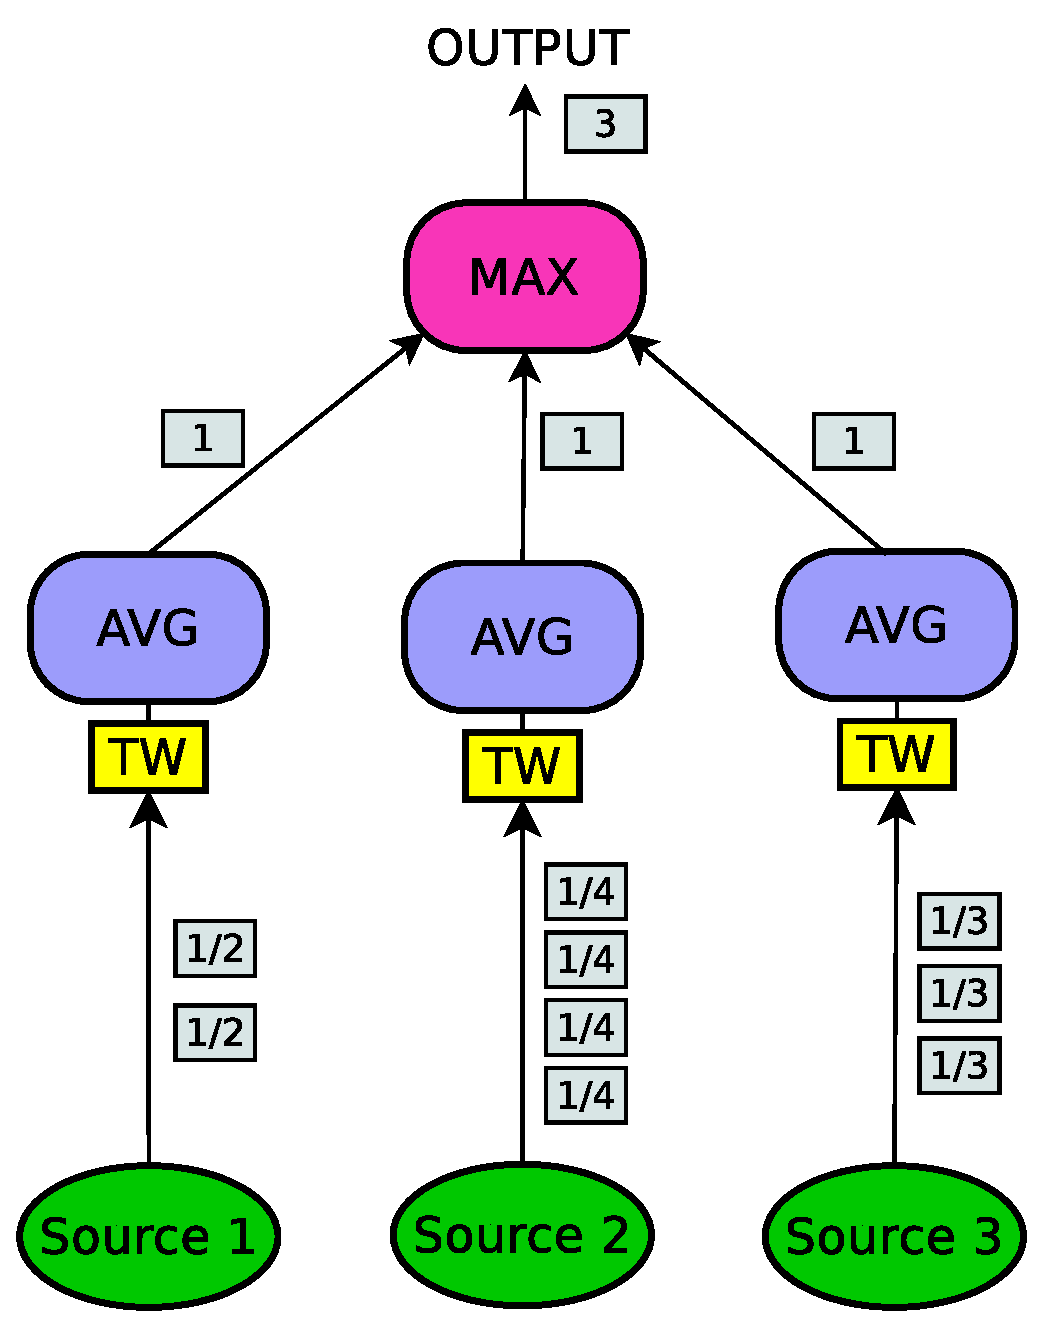
\includegraphics[width=0.35\textwidth]{img/tesi/query_fanin} \caption{An example of fan-in query. Input values for each source are first averaged over a certain time window, and
then the maximum value is selected. Source Coverage Ratio values are shown for each tuple.}
\label{fig:query_fanin2}
\end{figure}

The \textit{average} operator takes in input a batch of tuples of size 2, 3 and 4, respectively, and
outputs a single tuple. Assumption 6 (Conservation of Information) requires that the amount of
information going into an operator is equal to the amount in the output. Therefore, the newly generated
tuples are all assigned a \sic value of 1, which is the sum of the individual \sic values of the input
tuples.

The final \textit{max} operator inputs 3 tuples, each with a \sic value of 1, and outputs a single
tuple with a \sic value of 3. Even though the processing semantics of the max and average operators are
different, the calculation of \sic values remains the same, as required by Assumption 3 (A Generic
Metric).
The final tuple contains the total amount of information carried by all the initial input tuples. 

Let us consider what would happen to the final \sic value in case of the loss of a tuple, for example, a
source tuple produced by Source 2. In this case, the amount of information in the tuple generated by the
central average operator would be $3/4$ instead of $1$. The loss of information (\ie to the amount
of $1/4$) would then be propagated to the final tuple, which would have a \sic value of $11/4$ instead of
$3$.
Since the calculation of the \sic values is additive, the amount of information missing, compared to
the maximum value, is equal to the sum of the \sic values of the individual tuples that
were lost during processing.

\subsection*{Fan-out Queries}

\textbf{Split Computation Queries.} Figure~\ref{fig:fanout_mr} shows a query that processes 300 messages
during a time window. Each message is analysed by a Natural Language Processing (NLP) operator that calculates a
coefficient based on its text. Finally, a max operator outputs the message with the highest coefficient. 

We assume that the NLP operator is computationally intensive and would overload a single node at the
current rate. Therefore the computation is split across 3 different nodes. Each node processes 1/3 of
the messages, and all nodes manage to process all the messages without the need to discard data.
The \textit{split} operator creates a partition of the original stream without data
duplication, which means that the tuples that it outputs still have the same \sic value as the ones in
the input.

This follows from Assumption 9 (Queries are DAGs). In this query, the split operators receive as input
300 tuples. Each with a \sic value of 1/300.  The operator outputs 100 tuples on each output stream,
again with an individual \sic value of 1/300. Each stream is sent to a different processing node where a
NLP operator assigns a coefficient to each message. These operators output the same number of tuples
that they receive as input, thus producing 100 tuples each with an individual \sic value of 1/300.
Finally, all the tuples are processed by a Top-10 operator, which outputs the 10 tuples with the
highest coefficients. Each output tuple has a \sic value of 1/10, for a total final \sic value~of~1.

\begin{figure}[t!]
	\centering 
	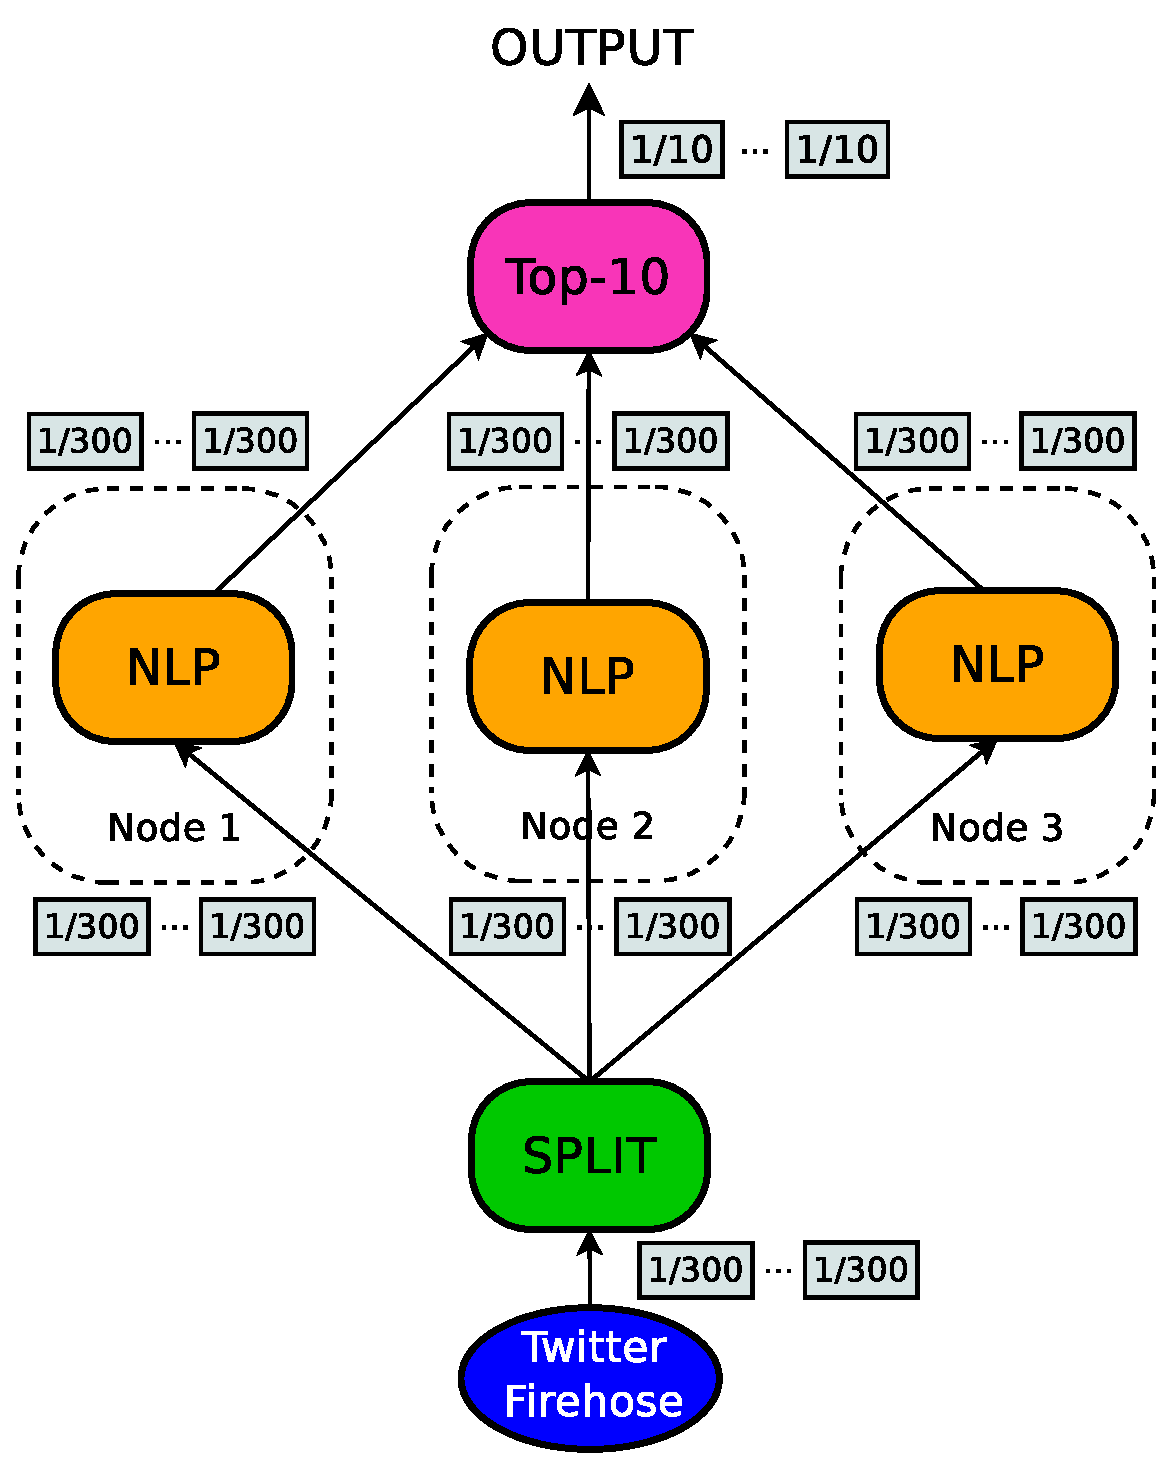
\includegraphics[width=0.5\textwidth]{img/tesi/fan-out_mr} 
	\caption{An example of a fan-out query processing Twitter data. 
	The Source Coverage Ratio values are shown for each tuple.}
	\label{fig:fanout_mr}
\end{figure}
\vspace{15pt}
\textbf{Multiple Results Queries.} Figure~\ref{fig:query_fanout} shows a query calculating the
occurrences of positive and negative mentions of a given keyword. 
This query computes 3 different results: the number of messages with a positive mention of a keyword,
the number of with a negative one and their ratio.
The original stream comes from the Twitter platform and contains an unsorted stream of messages. In our
example, during a time window, there are 3 messages with individual \sic values of 1/3. A filter
operator selects only those messages that contain a given keyword, in our example outputting 2
tuples.
At this point, the output of the filter operator is multiplexed over two different operators,
one that filters only messages with positive references to the keyword and one filtering negative
references.
\clearpage
\begin{figure}[t]
	\centering
	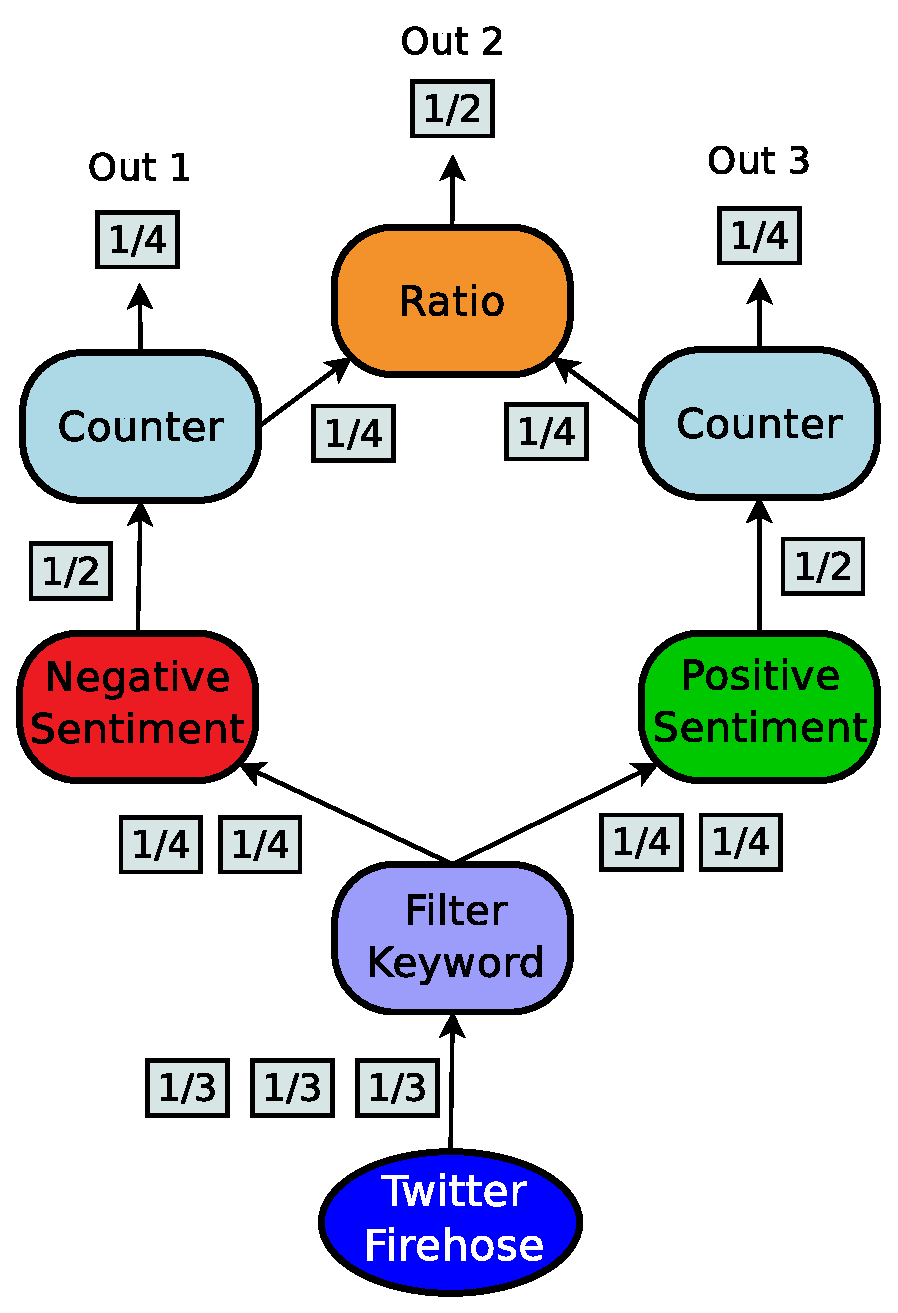
\includegraphics[width=0.45\textwidth]{img/tesi/fan-out_2} 
	\caption{An example of fan-out query processing Twitter data. It counts the occurrences of positive and
	negative mentions of a given keyword. The numbers shown on tuples are their individual \sic values.}
	\label{fig:query_fanout}
\end{figure}

Assumption 9 (Queries are DAGs) requires that, when such a duplication of the
output occurs, the total \sic value must be distributed over all output tuples. This is also in
accordance with Assumption 6 (Information Conservation) because the amount of information in the input is
equal to the amount in the output.
Each output stream of the \emph{keyword filter} operator contains an identical set of 2
tuples, each with an individual \sic value of 1/4.
The positive and negative filters each output a single tuple with a \sic value of 1/2. 

These output tuples propagate to \emph{counter} operators. These operators produce 2 output
streams: one that is terminal and is delivered as a result and another that feeds into a \emph{ratio}
operator.
Again the output of the counter operators is multiplexed and thus the individual \sic values of
the produced tuples are scaled accordingly. In our example, each counter produces 2 identical batches of
1 tuple with a \sic value of 1/4. The ratio operator outputs the third result of the query, producing a
single tuple with a \sic value of 1/2.
The result tuples have different \sic values: 1/4 for the
ones produced by the counter operators and 1/2 the ones produced by the ratio operator. If we sum
these together, we obtain a total \sic value of 1 for the query, which indicates that
no failure occurred during processing. 


